% !TeX root = Jumppanen.tex
\title{Introduction to \pkg{BuildSys}: An R Package for Compiling and Debugging R Dynamic Libraries}
\author{by Paavo Jumppanen}

\maketitle

\abstract{%
A powerful feature of \strong{R} is the ability to make use of dynamically loaded libraries and call functions within (API) through the \code{.C} or \code{.CALL} interface. 
This allows the numerically intensive parts of an algorithm to be implemented in efficient compiled code (typically \strong{C/C++} or \strong{FORTRAN}) to  
obtain a significant boost in performance. The flip side of this approach is the complexity and difficulty of compilation, and in particular,
the debugging of the compiled code. \pkg{BuildSys} is a package that streamlines and integrates into \strong{R}, the process of both building and debugging
dynamically loaded libraries using well established and freely available tools and making debugging in particular, a more pleasant and 
productive part of the process.  
}

\hypertarget{introduction}{%
\subsection{Introduction}\label{introduction}}
The process of producing functionally correct dynamic libraries for \strong{R} can be broken down into three processes: (1) code compilation to produce object files,
(2) linking object files to produce a dynamically library and (3) runtime testing and debugging of the library code. In \strong{R} steps (1) and (2) 
are typically handled through the \samp{R CMD SHLIB}\citep{SHLIB} mechanism. Internally that mechanism typically relies on \dfn{GNU make}\citep{GnuMake} which 
in turn will typically use \dfn{GCC}\citep{gcc} (on most operating systems) or \dfn{CLANG/LLVM}\citep{LLVM} (on MacOS). On Windows based systems \dfn{GNU make} and \dfn{GCC}
are used and are made available by the \dfn{MINGW} based \dfn{Rtools} installation\citep{UsingRtools}. Compilation through \samp{R CMD SHLIB} 
involves the use of a generic makefile bundled within the \strong{R} installation that in turn uses environment variable string substitutions to specify the details 
of which files and compiler switches are needed. The command itself takes the command line and translates it into a suitable call to GNU make with the correct 
environment variables to obtain the desired compilation result. This is a simple, effective and portable way to handle compilation of shared 
libraries within \strong{R} packages, but for general use in circumstances where there are compile and/or link errors due to makefile mis-configuration 
(ie. missing include paths, library paths or libraries), it can be challenging to determine the source of the error in the command line specification. Furthermore, 
if the shared library contains many individual source files and uses of a number of static third party libraries, the required command line can become 
unwieldy and may also require the use of a secondary \emph{Makevars} file to specify addition compiler switches. For one off library development that is not targetting
packaging deployment but simply fulfilling a one off need, it can be easier to address the build issues in compiling a library by using a project specific makefile 
and \dfn{GNU make} invocation directly rather than going through the \samp{R CMD SHLIB} mechanism. \pkg{BuildSys} takes this approach by encapsulating a makefile within 
an S4 class that is managed from within \strong{R}. 

The third process in library development, debugging, is the most cumbersome part of currently used approaches and remains a stumbling 
block for many wishing to develop custom dynamic libraries, but who lack the knowledge and experience to make use of the available debugging 
tools to do so. The most commonly used debugger in an \strong{R} context is \dfn{GDB}\citep{GDB}, which provides realtime debugging of the dynamic library within the
host application (\strong{R}) via a large set of command line commands invoked at a command prompt in \dfn{GDB}. Similarly, debugging in \strong{R} on MacOS is performed using another 
command line based debugger, \dfn{LLDB}\citep{LLDB}. 

If users manage to build the library with appropriate debug information included, load the hosting \strong{R} session, have the debugger find and 
load the symbol table information and set active breakpoints, then they are part way to being able to successfully debug their library. However, 
one major issue remains that has to do with inspection of variables and other data structures. By default, both \dfn{GDB} and \dfn{LLDB} only 
know how to display intrinsic data types (bool, char, int, double etc.) in a meaningful way via their respective watch commands. To be able to 
display variables of a complex data type (structures or classes) they both must be provided with custom print code to visualise those complex 
data types. They both can display nominal information about complex data types but the default display of such types is non-intuitive, not particularly informative
and cumbersome to work with. This only magnifies in cases of indexing arrayed complex data types. It is this limitation that is the fundamental stumbling block for 
debugging code that leads to resorting to debugging via print statements rather than the employment of a debugger. 

If library developers only rely on native data types then this will not be an issue, however doing so implicitely requires the use of \code{.C} or 
\code{.CALL} mechanisms directly; see for instance \citep{DotC} and \citep{DotC2}. This in turn requires an intimate
knowledge of how \strong{R} natively represents data structures internally, which can be intimidating to the less experienced programmer. A more common approach is to 
use a C++ library that encapsulates the native \strong{R} data structures within complex data types, of which both \dfn{GDB} and \dfn{LLDB} are  
incapable of meaningfully visualising in their default state. 

The most widely used interface wrapper within the \strong{R} community is \pkg{Rcpp}\citep{RcppIntro},\citep{Rcpp}. Additionally, the packages \pkg{RcppEigen} 
and \pkg{TMB} build upon that interface to support \emph{linear algebra} \citep{RcppEigen}, \citep{RcppEigenLA}, \emph{automatic differentiation} \citep{TMBlaplace} and 
\emph{random effects models} \citep{TMB}. The utility of these packages alone represent a clear motivation for developing support for a more complete debugging 
experience. In fact, the initial motivation in developing \pkg{BuildSys} was to aid in debugging \pkg{TMB} based random effects model development in a 
\emph{fisheries MSE} (management strategy evaluation) context, although the package has general utility in any \strong{R} dynamic library development situation.

\hypertarget{exitising-debugging-approaches}{%
\subsection{Existing Debugging Approaches}
\label{exitising-debugging-approaches}}
Despite being widely used, documentation relating to \pkg{Rcpp} is notable for the lack of mention in any significant way of the process of debugging. For instance, the 
introductory paper \emph{Extending R with C++: A brief Introduction to Rcpp} \citep{RcppIntro} makes no mention of debugging, nor does the package documentation \citep{Rcpp}. 
This equally applies to packages that build upon \pkg{Rcpp}. Anecdotally, debugging appears to be the \emph{bain of existence} of an \strong{R} library developer and 
there appears to be ample need for simpler (but not at the expense of capability) approaches. \citep{DebuggingRandCcodeinR} advocates debugging using 
\dfn{GDB}\citep{GDB}, either through \dfn{EMACS} or \dfn{DDD}\citep{DDD} as a \dfn{GDB} front end, with memory errors being tackled with \dfn{valgrind}\citep{valgrind}. Similarly, 
\citep{DebuggingC_Cpp} advocates \dfn{GDB} or \dfn{LLDB} \citep{LLDB} (depending on the target operating system) for general debugging and \dfn{valgrind} for debugging memory 
errors, though makes the point that \emph{this is not for the faint of heart, and requires some C-level familiarity}. Although not explicit, this hints at the difficulty
many experience with debugging dynamic libraries for R. Although not specifically related to R, \citep{ImprovingCppDebug} laments the mis-givings of the debugging experience 
(circa 2020), summarises existing approaches and proposes the use of \dfn{Microsoft Visual Code}\citep{VSCodeDownload} as a possible solution. A common feature of the 
GUI front end debuggers is the need for a non-trivial setup stage. \dfn{Microsoft Visual Code} is no exception, although \pkg{BuildSys} includes processes that fully automate
this setup stage, thereby making the process of GUI hosted debugging of R dynamic libraries simpler and more accessible.

\hypertarget{visual-studio-code-extensions}{%
\subsection{GUI Debugging though Visual Studio Code}
\label{visual-studio-code-extensions}}
\dfn{Visual Studio Code} is a freely available and extensible cross platform text editor designed specifically for coding. It has been widely adopted in the general programming
community with a user base in excess of 2.6 million\citep{VCusers} and was \emph{the number one project in the 2017 GitHub Octoverse}. Central to the 
popularity of the editor is the ability to customize it to particular niche needs through downloadable extensions. Of note in this particular application of \dfn{Visual Studio Code} 
is the \emph{Microsoft C/C++ extension} \citep{VSCodeCCppExt} which, apart from providing editor feature support targeting the C and C++ languages, also provides support for 
debugging via the machine interface to \dfn{GDB} (\dfn{GDB-MI}). It also provided debugging support on \dfn{MacOS} via \dfn{LLDB-MI}, however Apple have since abandoned support for \dfn{LLDB-MI} making 
the debugging support via this extension on MacOS inopperable. However, a third party extension, \dfn{CodeLLDB}\citep{CodeLLDB}, provides the equivalent debugging support that does not rely on
\dfn{LLDB-MI} to interface with \dfn{LLDB} and works with current versions of \dfn{MacOS}. 

Both \emph{CodeLLDB} and the \emph{Microsoft C/C++ extension} make debugging available through added configurations. These are codified using \dfn{JSON}\citep{JSON} format configration files;
one to specify how to launch or attach a debug session (the \emph{launch.json} file) and one to specify information needed to be able to correctly interpret the code within the debugging 
session (the \emph{c\_cpp\_properties.json} file). Typical \emph{launch.json} and \emph{c\_cpp\_properties.json} files are illustrated in Figures \ref{fig:launchJSON} and \ref{fig:CnCppProp}.
Whilst not overly complex, it is relatively easy to mis-configure and be left with partially operable or completely broken debugging. In the case of \pkg{BuildSys} these two files are 
automatically generated for the user and placed in the necessary folder so no user intervention is required and debugging works as expected.

Within a \emph{Visual Code} debug session (Figure \ref{fig:VisualCode}) the user has the ability to:

\begin{itemize}
\item set breakpoints either with or without conditions (ie. breakpoint counts and breakpoints triggered by data expression)
\item control execution flow with, single stepping, stepping in and stepping out
\item add variable watches to the watch window
\item see contexual local variable data
\item see the stack frame and navigate through the call trace
\end{itemize}

Of particular note is the ability to use complex evaluated expressions that update with program flow within the watch window (\code{xa[i]}, \code{xb[j]} in Figure \ref{fig:VisualCode}). 
Whilst a seasoned \dfn{GDB} or \dfn{LLDB} user could extract this information in the command line equivalent, multiple commands taken from a vast command set are typically required,
making this approach challenging for a novice user of these products. On the other hand, in a GUI presented interface the process of utilising these debugging features is made obvious, 
requires little understanding of the debugger command set, and presents the information in a readily digestible manner, making the debugging experience less daungting and more productive, 
particularly for the novice user. 

\begin{Schunk}
\begin{figure}[htbp]
{\centering}
\begin{verbatim}
{
  "version": "0.2.0",
  "configurations": [
    {
      "name": "(gdb) Launch",
      "type": "cppdbg",
      "request": "launch",
      "targetArchitecture":"x86_64",
      "program": "C:/Users/jum002/DOCUME~1/R/R-40~1.5/bin/x64/Rgui.exe",
      "args": ["--no-save", "--no-restore"],
      "stopAtEntry": false,
      "cwd": "C:/Users/jum002/DOCUME~1/Test/CONVOL~1.RPR",
      "environment": [{"name":"R_HOME",
                       "value":"C:/Users/jum002/Documents/R/R-4.0.5"}],
      "externalConsole": true,
      "MIMode": "gdb",
      "miDebuggerPath": "C:/rtools40/mingw64/bin/gdb.exe",
      "miDebuggerArgs": "--init-command debugCmd.txt",
      "setupCommands": [
        {
          "description": "Enable pretty-printing for gdb",
          "text": "-enable-pretty-printing",
          "ignoreFailures": true
        }
      ]
    }
  ]
}
\end{verbatim}
\caption[A Typical launch.json File]{A Typical launch.json File}
\label{fig:launchJSON}
\end{figure}
\end{Schunk}
  
\begin{Schunk}
\begin{figure}[htbp]
{\centering}
\begin{verbatim}
{
  "configurations": [
  {
    "name": "Win32",
    "intelliSenseMode": "gcc-x64",
    "includePath": ["${workspaceFolder}",
                    "C:/rtools40/mingw64/include/**",
                    "C:/rtools40/usr/include/**",
                    "C:/Users/jum002/DOCUME~1/R/R-40~1.5/include/**",
                    "C:/Users/jum002/DOCUME~1/Test/**",
                    "C:/Users/jum002/DOCUME~1/R/R-40~1.5/include/**"],
    "defines": [],
    "compilerPath": "C:/rtools40/mingw64/bin/gcc.exe",
    "cStandard": "c89",
    "cppStandard": "c++14",
    "browse": {
        "limitSymbolsToIncludedHeaders": true,
        "databaseFilename": ""
      }
    }
  ],
  "version": 4
}
\end{verbatim}
\caption[A Typical c\_cpp\_properties.json File]{A Typical c\_cpp\_properties.json File}
\label{fig:CnCppProp}
\end{figure}
\end{Schunk}
  
\begin{Schunk}
\begin{figure}[htbp]
{\centering 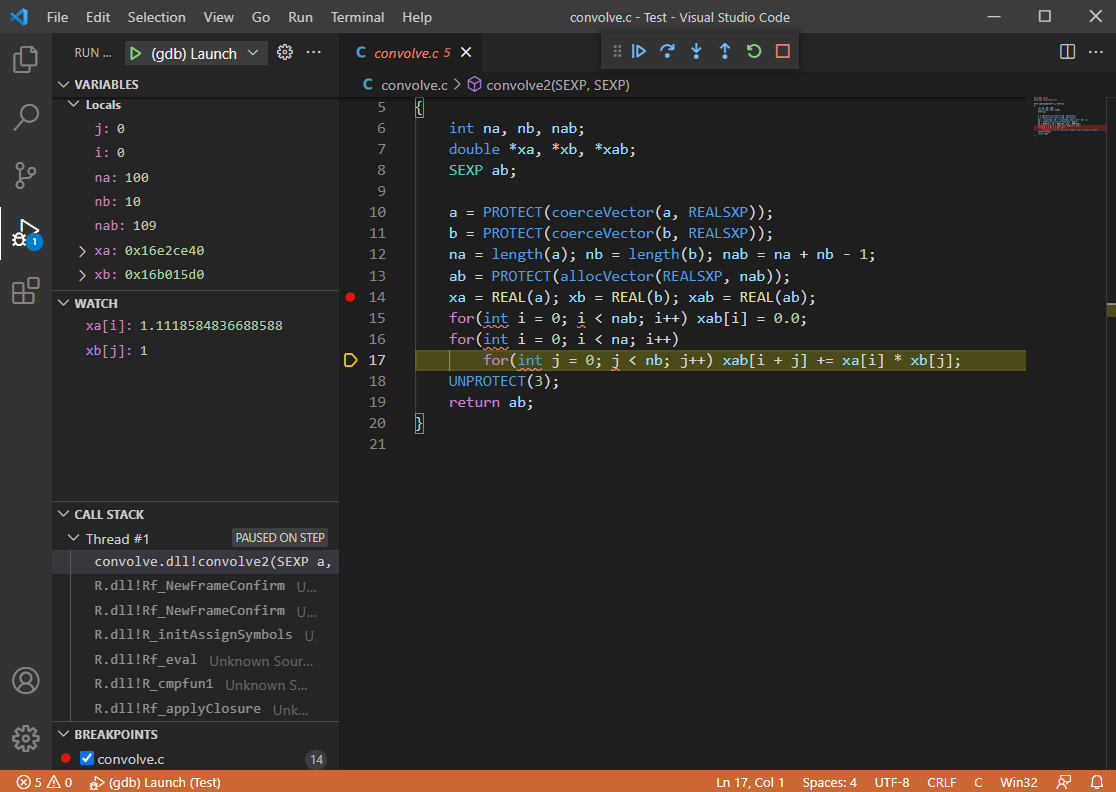
\includegraphics[width=0.95\textwidth]{VisualCode} 

}
\caption[Visual Code Debug Session]{Visual Code Debug Session}\label{fig:VisualCode}
\end{figure}
\end{Schunk}

Introductory section which may include references in parentheses
\citep{R}, or cite a reference such as \citet{R} in the text. \citep{Rcpp}, \citep{RcppEigen}, \citep{TMB}, \citep{Rextensions}
\citep{DebuggingC_Cpp},\citep{DebuggingRandCcodeinR}, \citep{CodeLLDB-manual}, \citep{CodeLLDB}, \citep{VSCodeTipsTricks}, 
\citep{VSCodeDownload}, \citep{VSCodeCCppExt}, \citep{VSCodeCCpp}, \citep{GDB}, \citep{ModernDebugging}, \citep{DDD},
\citep{ImprovingCppDebug},\citep{UsingRtools}, \citep{RcppIntro}, \citep{ihaka:1996}, \citep{RcppEigenLA},
\citep{TMBlaplace},\citep{DotC},\citep{DotC2},\citep{deSolve},\citep{Routines},\citep{LLDB},
\citep{Xcode},\citep{debug-visualize-ext},\citep{debug-visualize}

\hypertarget{section-title-in-sentence-case}{%
\subsection{Section title in sentence
case}\label{section-title-in-sentence-case}}

%This section may contain a figure such as Figure \ref{fig:Rlogo}.
%
%\begin{Schunk}
%\begin{figure}[htbp]
%
%{\centering \includegraphics[width=2in]{Rlogo} 
%
%}

%\caption[The logo of R]{The logo of R.}\label{fig:Rlogo}
%\end{figure}
%\end{Schunk}

%\hypertarget{another-section}{%
%\subsection{Another section}\label{another-section}}

There will likely be several sections, perhaps including code snippets,
such as:

%\begin{Schunk}
%\begin{Sinput}
%x <- 1:10
%plot(x)
%\end{Sinput}
%
%\includegraphics{Journal_files/figure-latex/unnamed-chunk-1-1} \end{Schunk}
%
%\hypertarget{summary}{%
%\subsection{Summary}\label{summary}}

This file is only a basic article template. For full details of
\emph{The R Journal} style and information on how to prepare your
article for submission, see the
\href{https://journal.r-project.org/share/author-guide.pdf}{Instructions
for Authors}.

\hypertarget{about-this-format-and-the-r-journal-requirements}{%
\subsubsection{About this format and the R Journal
requirements}\label{about-this-format-and-the-r-journal-requirements}}

\texttt{rticles::rjournal\_article} will help you build the correct
files requirements:

\begin{itemize}
\tightlist
\item
  A R file will be generated automatically using \texttt{knitr::purl} -
  see \url{https://bookdown.org/yihui/rmarkdown-cookbook/purl.html} for
  more information.
\item
  A tex file will be generated from this Rmd file and correctly included
  in \texttt{RJwapper.tex} as expected to build \texttt{RJwrapper.pdf}.
\item
  All figure files will be kept in the default rmarkdown
  \texttt{*\_files} folder. This happens because
  \texttt{keep\_tex\ =\ TRUE} by default in
  \texttt{rticles::rjournal\_article}
\item
  Only the bib filename is to modifed. An example bib file is included
  in the template (\texttt{RJreferences.bib}) and you will have to name
  your bib file as the tex, R, and pdf files.
\end{itemize}

\bibliography{BuildSysReferences.bib}

\address{%
Paavo Jumppanen\\
CSIRO Marine and Atmospheric Research\\%
Castray Esplanade,\\Battery Point TAS 7004,\\Australia\\
%
\url{https://www.csiro.au}%
\\\href{mailto:paavo.jumppanen@csiro.au}{\nolinkurl{paavo.jumppanen@csiro.au}}
}
